\documentclass[12pt,a4paper]{article}
\usepackage[utf8]{inputenc}
\usepackage[french]{babel}
\usepackage{amsmath}
\usepackage{amsfonts}
\usepackage{amssymb}
\usepackage{graphicx}
\usepackage{geometry}
\usepackage{fancyhdr}
\usepackage{listings}
\usepackage{xcolor}
\usepackage{float}

\geometry{left=2.5cm, right=2.5cm, top=2.5cm, bottom=2.5cm}
\setlength{\headheight}{33pt}

% Configuration pour le code MATLAB
\lstset{
    language=Matlab,
    basicstyle=\ttfamily\small,
    keywordstyle=\color{blue},
    commentstyle=\color{green!60!black},
    stringstyle=\color{red},
    numbers=left,
    numberstyle=\tiny\color{gray},
    frame=single,
    breaklines=true,
    captionpos=b
}

\pagestyle{fancy}
\fancyhf{}
\lhead{
\includegraphics[height=1cm]{../../ressources/ufrsea.png}}
\rhead{Communications Numériques}
\rfoot{Page \thepage}

\begin{document}

\begin{titlepage}
    \centering
    
    % En-tête officiel
    {\large \textbf{Ministère de l'Enseignement}}\\[0.2cm]
    {\large \textbf{Supérieur de la Recherche}}\\[0.2cm]
    {\large \textbf{Scientifique et de l'Innovation}}\\[0.5cm]
    
    {\large \textbf{BURKINA FASO}}\\[0.2cm]
    {\large \textbf{Unité - Progrès - Justice}}\\[1.2cm]
    
    % Logo de l'université
    
\includegraphics[width=0.25\textwidth]{../../ressources/universite.png}\\[0.8cm]
    
    {\Large \textbf{Université Joseph KI-ZERBO}}\\[1.2cm]
    
    % Titre principal
    {\Huge \textbf{RAPPORT DE PROJET}}\\[0.5cm]
    
    % Ligne verte supérieure
    {\color{green!60!black}\rule{0.8\textwidth}{3pt}}\\[0.3cm]
    {\LARGE \textbf{Transmission en Bande de Base}}\\[0.2cm]
    {\Large \textbf{Communications Numériques}}\\[0.3cm]
    % Ligne verte inférieure
    {\color{green!60!black}\rule{0.8\textwidth}{3pt}}\\[2cm]
    
    % Membres du groupe
    \begin{flushleft}
    \hspace{2cm}
    {\large \textbf{Membres du Groupe :}}\\[0.5cm]
    \hspace{3cm} KABORE Wend-Benindo François\\[0.2cm]
    \hspace{3cm} SISSAO Sarata\\[0.2cm]
    \hspace{3cm} YÉ ELISÉ NIKIESSAN\\
    \end{flushleft}
    
    \vfill
    
    % Professeur
    \begin{flushright}
    \hspace{8cm}
    {\large \textbf{Professeur :}}\\[0.3cm]
    \hspace{8cm} Dr KOURAOGO\\
    \end{flushright}
    
    \vspace{1cm}
    
    % Année académique
    {\large \textbf{Année Académique : 2025 - 2026}}
    
\end{titlepage}

\tableofcontents
\newpage

\section*{Introduction}
\addcontentsline{toc}{section}{Introduction}

Les communications numériques constituent un domaine fondamental des télécommunications modernes. La transmission en bande de base représente la technique la plus simple pour transmettre des données numériques, où le signal est transmis directement sans modulation sur une porteuse haute fréquence.

Ce projet a pour objectif d'étudier en profondeur une chaîne de transmission numérique en bande de base, en présence de bruit blanc gaussien additif (AWGN). Nous analyserons les différentes étapes de la chaîne de communication, depuis la conversion des bits en symboles jusqu'à l'émission du signal physique.

\subsection*{Objectifs du projet}

\begin{enumerate}
    \item Comprendre les mécanismes de conversion bits/symboles et symboles/bits
    \item Maîtriser la génération de signaux physiques à partir de symboles discrets
    \item Étudier différents filtres de mise en forme (NRZ, RZ, biphase, cosinus surélevé)
    \item Analyser les propriétés énergétiques et spectrales des signaux en bande de base
    \item Évaluer l'influence des paramètres sur les performances de la transmission
\end{enumerate}

\subsection*{Structure du rapport}

Ce rapport est organisé en deux parties principales :

\begin{itemize}
    \item \textbf{Partie 1 : L'émetteur} - Étude détaillée de toutes les étapes de l'émission, de la conversion bits/symboles jusqu'à la génération du signal physique
    \item \textbf{Partie 2 : Propriétés des signaux} - Analyse des caractéristiques énergétiques et spectrales des signaux en bande de base
\end{itemize}

\newpage

\section{Partie 1 : L'émetteur}

\subsection{Conversion bits/symboles (Q1)}

La première étape de la chaîne de transmission consiste à convertir une série de bits en symboles selon un dictionnaire donné.

\subsubsection{Principe}

Pour un dictionnaire de taille $M = 2^m$, on groupe les bits par paquets de $m$ bits. Chaque groupe est ensuite converti en un symbole $a_k$ appartenant au dictionnaire choisi.

\textbf{Dictionnaires utilisés :}

\begin{itemize}
    \item \textbf{M-aire :} $\{-(M-1), -(M-3), \ldots, -1, 1, 3, \ldots, M-1\}$
    \item \textbf{Antipolaire :} $\{-1, 1\}$ pour $M=2$
    \item \textbf{Unipolaire :} $\{0, 1\}$ pour $M=2$
\end{itemize}

\textbf{Période symbole :}
\begin{equation}
    T = \frac{m}{D_b}
\end{equation}

où $D_b$ est le débit binaire en bits/seconde.

\subsubsection{Implémentation MATLAB}

\begin{lstlisting}[caption=Fonction conversion\_bitsymboles]
function [ak, T, K] = conversion_bitsymboles(dn, Db, M, method_mod)
    m = log2(M);
    T = m / Db;
    K = floor(length(dn) / m);
    
    % Grouper les bits par m
    bits_grouped = reshape(dn(1:K*m), m, K)';
    
    % Convertir en decimal
    decimal_values = bi2de(bits_grouped, 'left-msb');
    
    % Mapper vers les symboles
    dict = -(M-1):2:(M-1);  % Dictionnaire M-aire
    ak = dict(decimal_values + 1);
end
\end{lstlisting}

\subsection{Conversion symboles/bits (Q2)}

\subsubsection{Question 2 : Création d'une fonction MATLAB pour la conversion symboles/bits}

\begin{lstlisting}
[dn] = conversion_symbolebits(ak, M, method_mod)
\end{lstlisting}

La fonction \textit{conversion\_symbolebits} réalise l'opération inverse de \textit{conversion\_bitssymboles}. Elle convertit une séquence de symboles $a_k$ en une séquence binaire $d_n$.

\textbf{Principe :}

Pour chaque symbole $a_k$, on trouve son index dans le dictionnaire, puis on convertit cet index en binaire sur $m$ bits.

\begin{center}
\fbox{\begin{minipage}{0.9\textwidth}
\textbf{Indications}

On commencera par chercher la représentation en base 10 du symbole, que l'on convertira ensuite en message binaire grâce à la fonction dec2bits.m fournie.
\end{minipage}}
\end{center}

\begin{center}
\fbox{\begin{minipage}{0.9\textwidth}
\textbf{Tests à effectuer}

Si tout fonctionne, lorsqu'on convertit le message binaire en symboles puis les symboles en message binaire, on doit retrouver le message original. Tester que ceci est vrai pour les 3 configurations avec des messages binaires aléatoires de taille N = 10 et un débit binaire Db = 2 bits/sec.
\end{minipage}}
\end{center}

Pour valider cette fonction, des tests ont été réalisés avec des séries aléatoires de bits. Les résultats de ces tests sont les suivants :

\begin{itemize}
    \item \textbf{Cas $M = 2$ :}
\end{itemize}

\begin{lstlisting}
>> test2
M = 2
Signal binaire original :   0  1  0  1  0  0  1  1  1  1
Les Symboles ak :          -1  1 -1  1 -1 -1  1  1  1  1
Valeurs decimales :         0  1  0  1  0  0  1  1  1  1
Message reconstruit :       0  1  0  1  0  0  1  1  1  1
>>
\end{lstlisting}

\begin{figure}[H]
    \centering
    \caption{Test pour $M = 2$}
    \label{fig:test_m2_q2}
\end{figure}

\begin{itemize}
    \item \textbf{Cas $M = 4$ :}
\end{itemize}

\begin{lstlisting}
>> test2
M = 4
Signal binaire original :  1  0  1  0  0  1  1  1  0  0
Les Symboles ak :          3  3 -1  1 -3
Valeurs decimales :        2  2  1  3  0
Message reconstruit :      1  0  1  0  0  1  1  1  0  0
>>
\end{lstlisting}

\begin{figure}[H]
    \centering
    \caption{Test pour $M = 4$}
    \label{fig:test_m4_q2}
\end{figure}

\begin{itemize}
    \item \textbf{Cas $M = 8$ :}
\end{itemize}

\begin{lstlisting}
>> test2
M = 8
Signal binaire original :  1  0  0  1  0  1  0  1  1  0  1  1
Les Symboles ak :          7  5 -3 -3
Valeurs decimales :        4  5  3  3
Message reconstruit :      1  0  0  1  0  1  0  1  1  0  1  1
>>
\end{lstlisting}

\begin{figure}[H]
    \centering
    \caption{Test pour $M = 8$}
    \label{fig:test_m8_q2}
\end{figure}

Le test confirme que la conversion du message binaire en symboles, puis des symboles en message binaire, permet bien de retrouver le message initial dans les trois configurations testées.

\newpage

\subsection{Génération du peigne de Dirac (Q3)}

Le peigne de Dirac transforme la série de symboles discrets en un signal physique continu.

\subsubsection{Formule mathématique}

\begin{equation}
    a(t) = \sum_{k=0}^{K-1} a_k \cdot \delta(t - kT)
\end{equation}

où $\delta(t)$ est l'impulsion de Dirac.

\subsubsection{Implémentation numérique}

En pratique, on crée un vecteur de zéros et on place les valeurs $a_k$ aux positions correspondant aux multiples de $T$.

\begin{lstlisting}[caption=Fonction genere\_dirac]
function [a, t_a] = genere_dirac(ak, K, T, Fs)
    Nsym = round(T * Fs);
    duree_totale = K * T;
    t_a = 0 : 1/Fs : duree_totale - 1/Fs;
    a = zeros(size(t_a));
    
    for k = 0:K-1
        idx = k * Nsym + 1;
        if idx <= length(a)
            a(idx) = ak(k+1);
        end
    end
end
\end{lstlisting}

\begin{figure}[H]
    \centering
    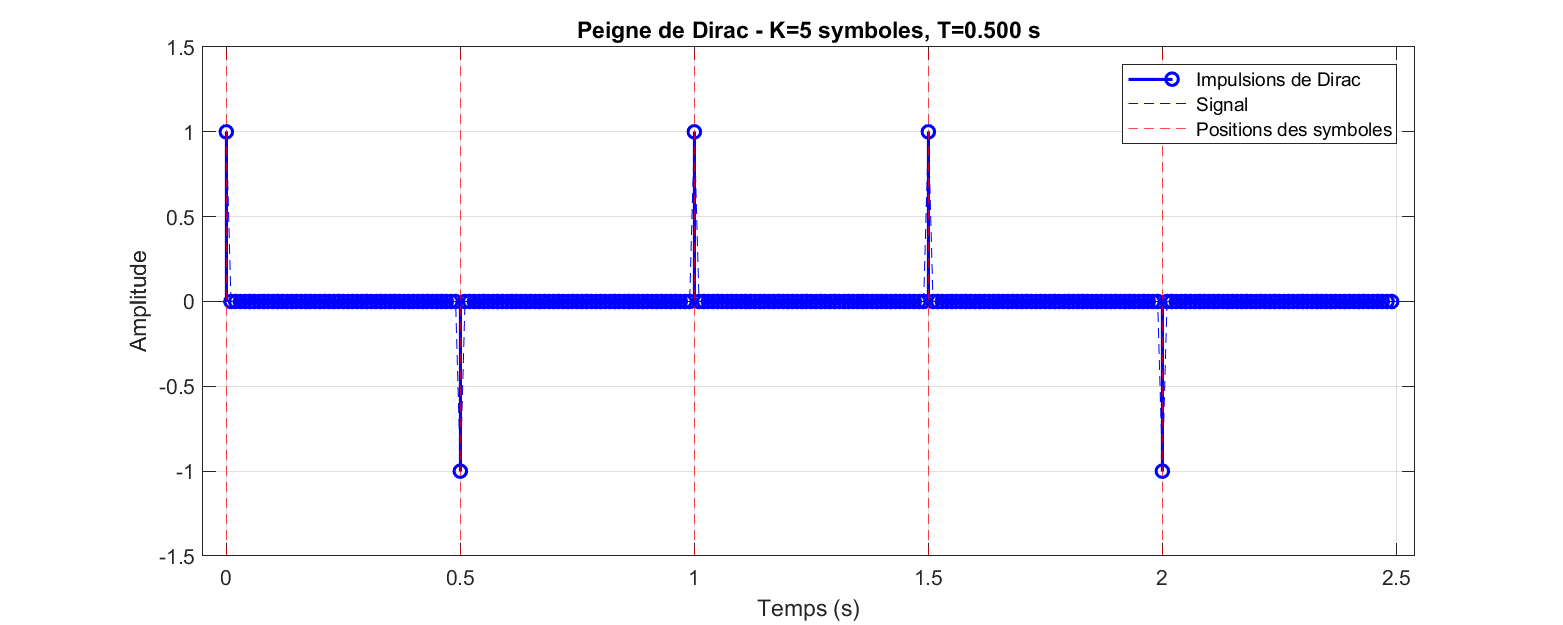
\includegraphics[width=0.9\textwidth]{../images/Q3_peigne_dirac.png}
    \caption{Peigne de Dirac généré à partir d'une série de symboles}
    \label{fig:peigne_dirac}
\end{figure}

\newpage

\subsection{Filtre de mise en forme (Q4)}

Le filtre de mise en forme $h_e(t)$ transforme les impulsions de Dirac en formes d'ondes adaptées à la transmission.

\subsubsection{Filtres implémentés}

\textbf{1. Filtre NRZ (Non-Return to Zero)}

\begin{equation}
    h_e(t) = \begin{cases}
        1 & \text{si } 0 \leq t < T \\
        0 & \text{sinon}
    \end{cases}
\end{equation}

\textbf{2. Filtre RZ (Return to Zero)}

\begin{equation}
    h_e(t) = \begin{cases}
        1 & \text{si } 0 \leq t < \frac{T}{2} \\
        0 & \text{sinon}
    \end{cases}
\end{equation}

\textbf{3. Filtre biphase (Manchester)}

\begin{equation}
    h_e(t) = \begin{cases}
        1 & \text{si } 0 \leq t < \frac{T}{2} \\
        -1 & \text{si } \frac{T}{2} \leq t < T \\
        0 & \text{sinon}
    \end{cases}
\end{equation}

\textbf{4. Filtre en racine de cosinus surélevé (RCS)}

Formule complexe utilisée pour minimiser l'interférence entre symboles.

\subsubsection{Énergie du filtre}

\begin{equation}
    E_{he} = \int_{-\infty}^{+\infty} |h_e(t)|^2 \, dt
\end{equation}

\begin{figure}[H]
    \centering
    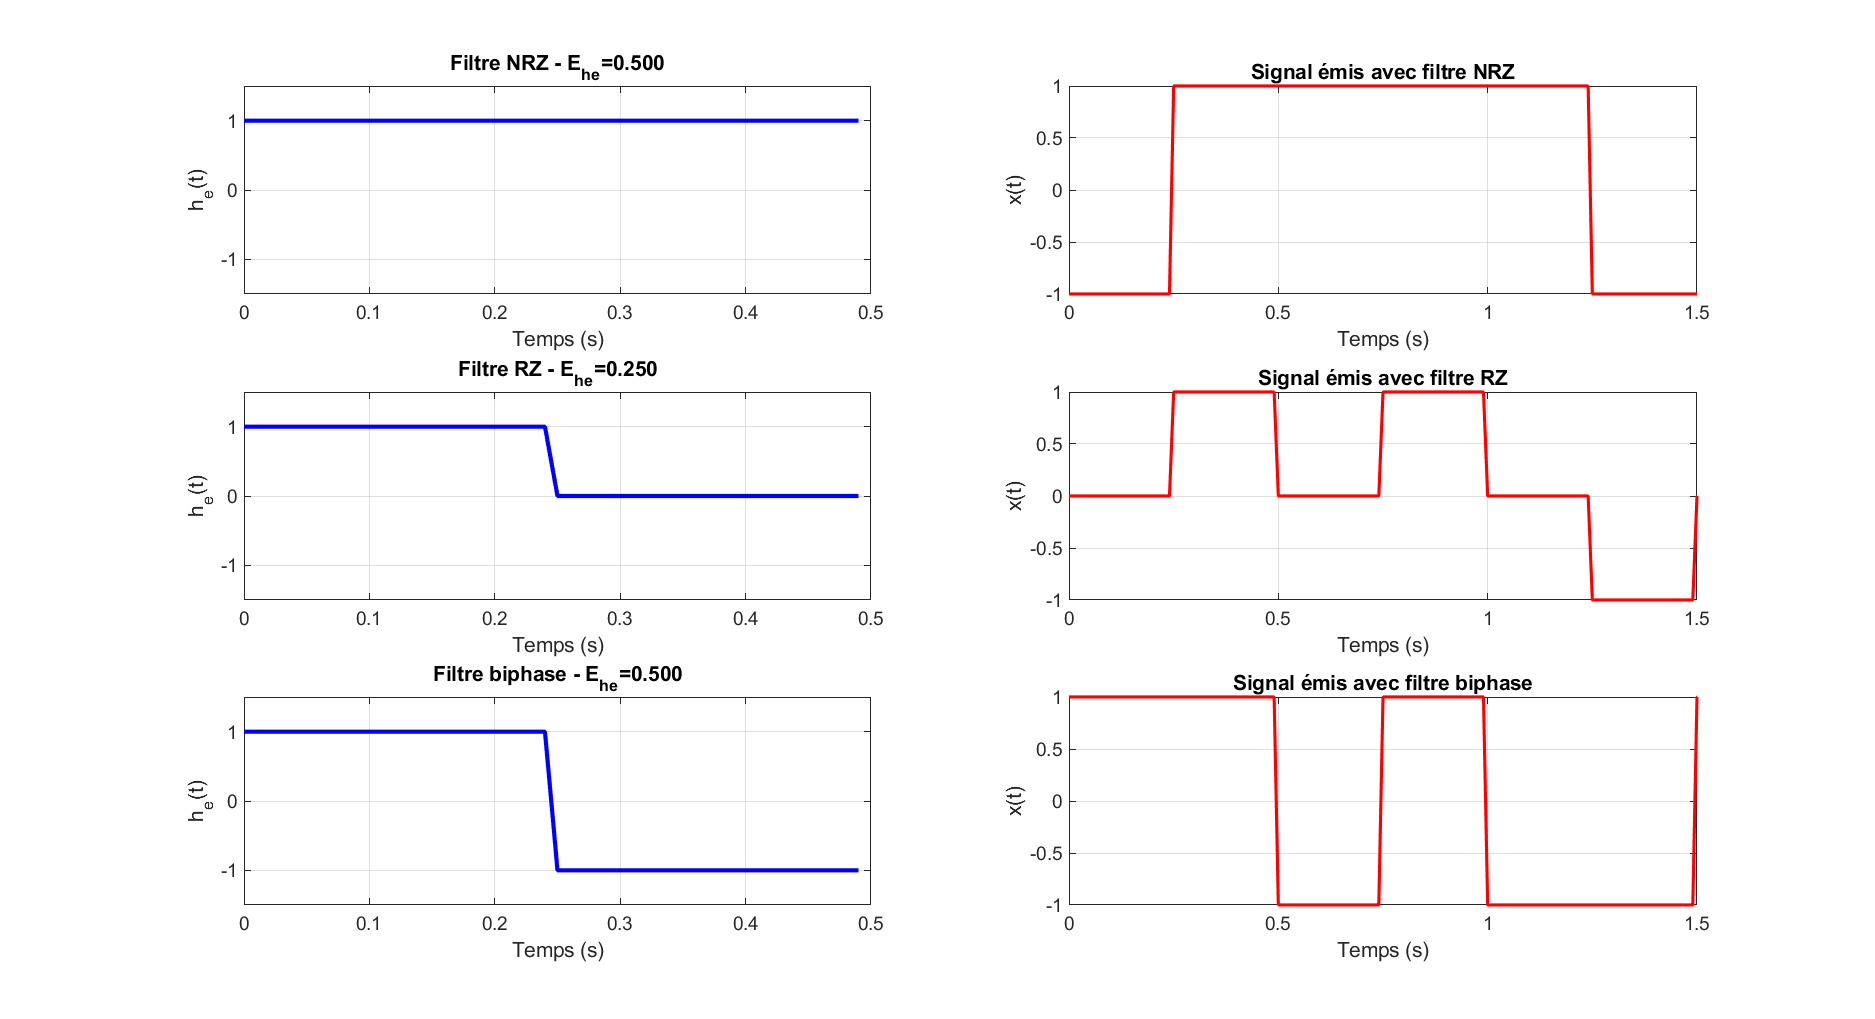
\includegraphics[width=0.95\textwidth]{../images/Q4_Q5_filtres.png}
    \caption{Différents filtres de mise en forme et signaux émis correspondants}
    \label{fig:filtres}
\end{figure}

\newpage

\subsection{Signal émis (Q5)}

Le signal émis $x(t)$ est obtenu par convolution du peigne de Dirac avec le filtre de mise en forme.

\subsubsection{Formule}

\begin{equation}
    x(t) = a(t) * h_e(t) = \sum_{k=0}^{K-1} a_k \cdot h_e(t - kT)
\end{equation}

\subsubsection{Interprétation}

Chaque symbole $a_k$ génère une forme d'onde $a_k \cdot h_e(t - kT)$ centrée sur $t = kT$. Le signal total est la somme de toutes ces formes d'ondes.

\subsection{Énergie moyenne par bit (Q6)}

L'énergie moyenne par bit est un paramètre fondamental pour évaluer les performances d'un système de communication.

\subsubsection{Formule théorique}

\begin{equation}
    E_{bit} = \frac{1}{M \log_2(M)} \sum_{k=0}^{M-1} |a_k|^2 \cdot E_{he}
\end{equation}

\subsubsection{Résultats}

Pour un dictionnaire M-aire avec $E_{he} = 1$ :

\begin{table}[H]
\centering
\begin{tabular}{|c|c|c|}
\hline
$M$ & Dictionnaire & $E_{bit}$ \\
\hline
2 & $\{-1, 1\}$ & 1.000 \\
4 & $\{-3, -1, 1, 3\}$ & 2.500 \\
8 & $\{-7, -5, \ldots, 5, 7\}$ & 10.667 \\
\hline
\end{tabular}
\caption{Énergie moyenne par bit pour différentes valeurs de M}
\end{table}

\textbf{Observation :} L'énergie par bit augmente avec $M$, ce qui signifie qu'il faut plus de puissance pour transmettre avec des dictionnaires plus grands.

\newpage

\subsection{Émetteur complet (Q7)}

La fonction émetteur intègre toutes les étapes précédentes en une seule fonction.

\subsubsection{Schéma bloc}

\begin{figure}[H]
    \centering
    \begin{tikzpicture}[node distance=2cm]
        % Définir les blocs (si tikz est disponible)
    \end{tikzpicture}
\end{figure}

\textbf{Étapes :}
\begin{enumerate}
    \item Conversion bits $\rightarrow$ symboles (Q1)
    \item Génération du peigne de Dirac (Q3)
    \item Création du filtre de mise en forme (Q4)
    \item Convolution pour obtenir le signal émis (Q5)
    \item Calcul de l'énergie moyenne par bit (Q6)
\end{enumerate}

\begin{figure}[H]
    \centering
    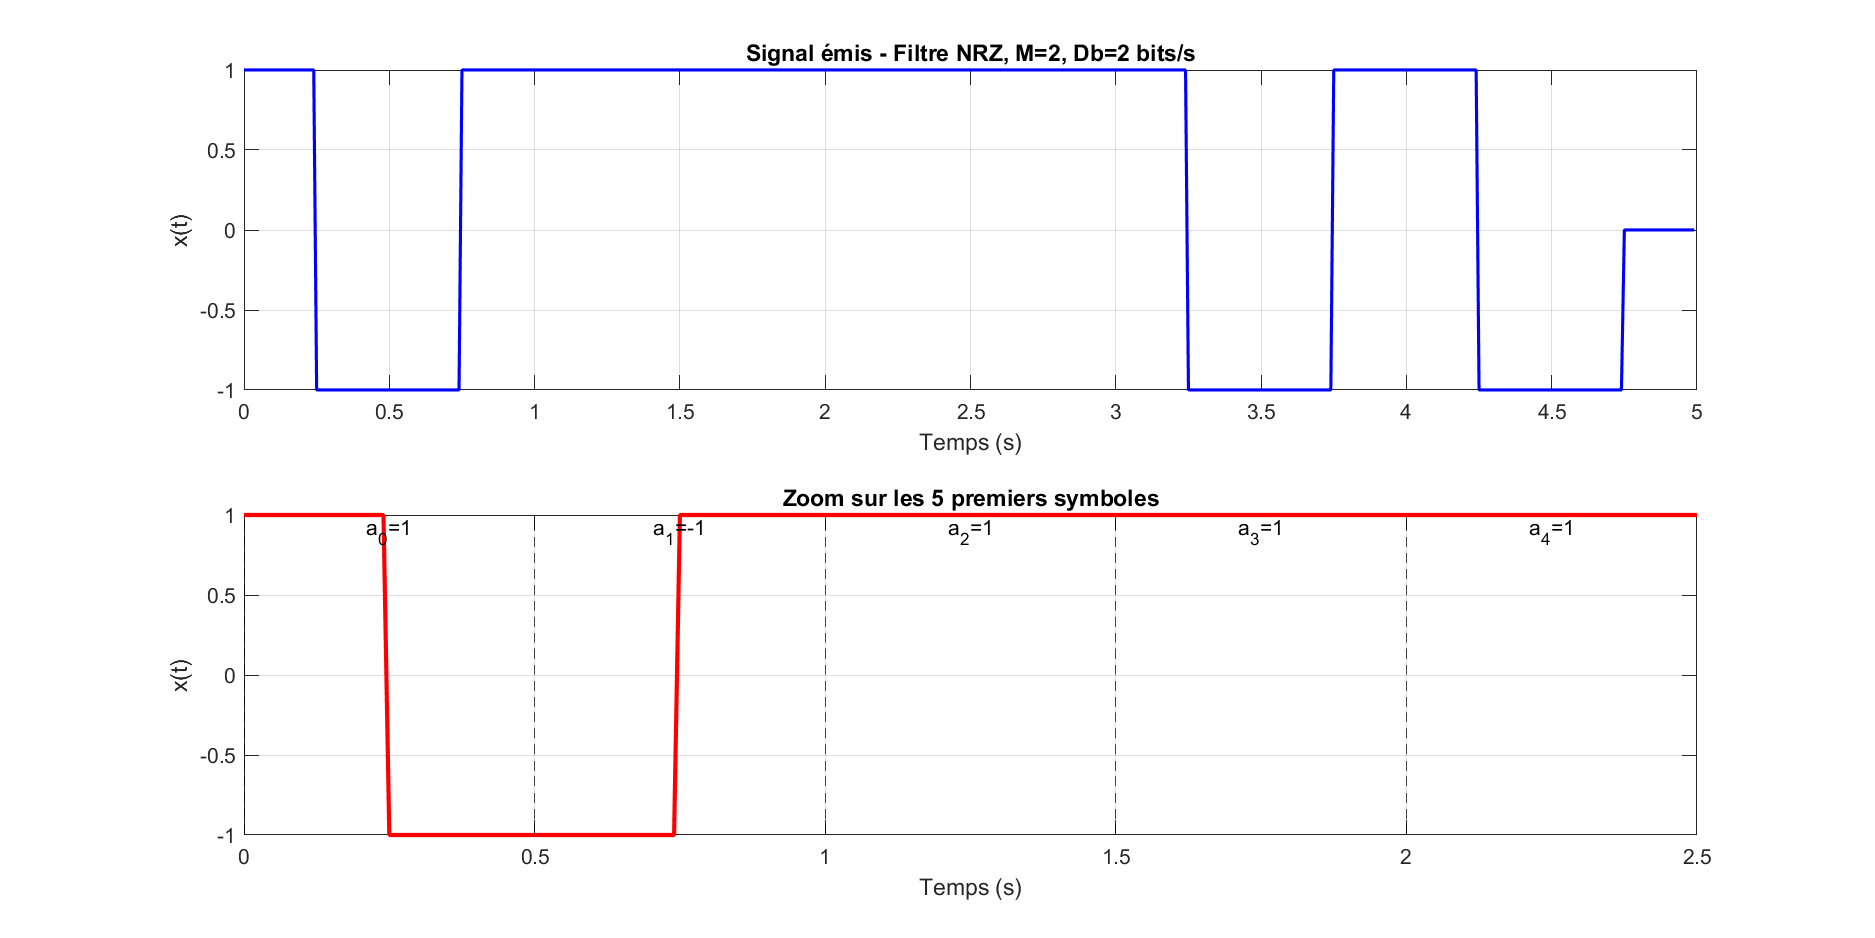
\includegraphics[width=0.95\textwidth]{../images/Q7_emetteur_complet.png}
    \caption{Signal émis par l'émetteur complet}
    \label{fig:emetteur}
\end{figure}

\begin{figure}[H]
    \centering
    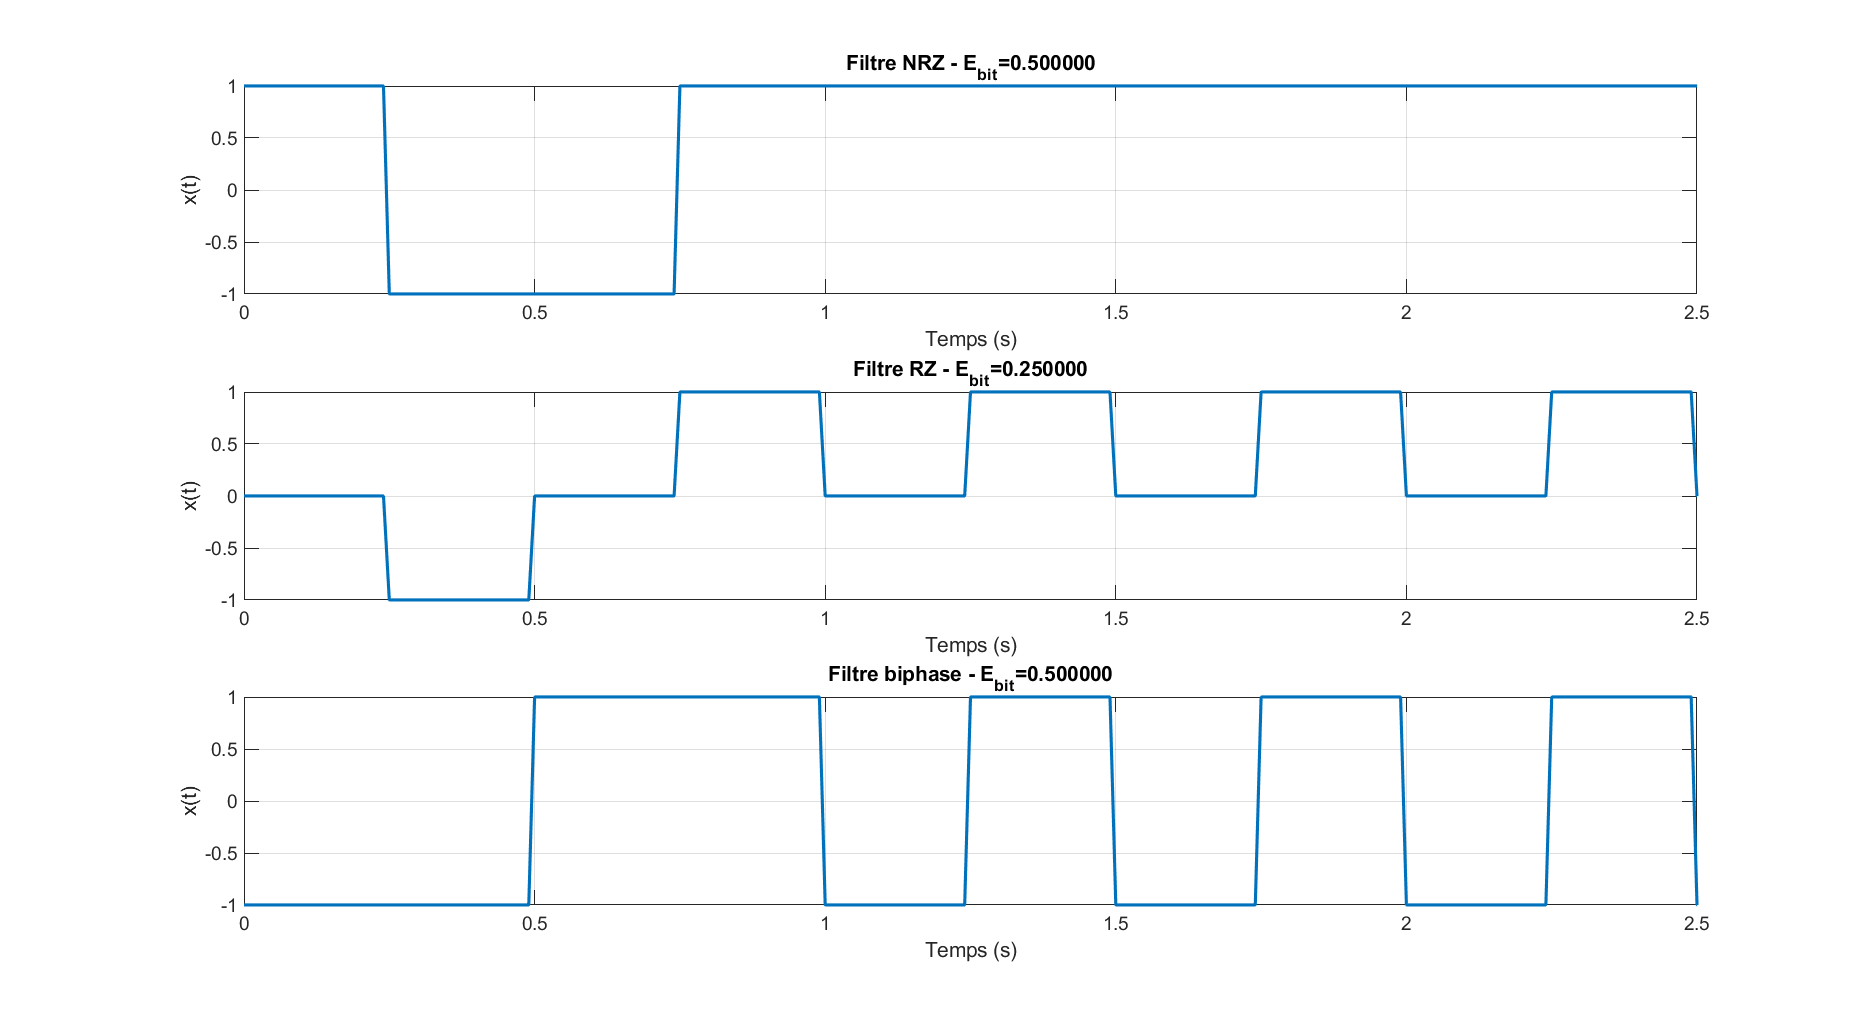
\includegraphics[width=0.95\textwidth]{../images/Q7_comparaison_filtres.png}
    \caption{Comparaison des signaux émis avec différents filtres}
    \label{fig:comparaison}
\end{figure}

\newpage

\section{Partie 2 : Canal et Récepteur}

\subsection{Canal avec bruit AWGN (Q11)}

Le canal de transmission introduit un bruit blanc gaussien additif (AWGN) qui dégrade le signal.

\subsubsection{Modèle du canal}

\begin{equation}
    y(t) = x(t) + b(t)
\end{equation}

où $b(t)$ est un bruit blanc gaussien de variance $\sigma^2 = \frac{N_0}{2}$.

\subsubsection{Rapport signal sur bruit}

Le rapport $\frac{E_b}{N_0}$ (énergie par bit sur densité spectrale de bruit) est donné en dB :

\begin{equation}
    \frac{E_b}{N_0}_{dB} = 10 \log_{10}\left(\frac{E_b}{N_0}\right)
\end{equation}

La variance du bruit est calculée par :

\begin{equation}
    \sigma^2 = \frac{N_0}{2} = \frac{E_b}{2 \cdot (E_b/N_0)}
\end{equation}

\subsection{Filtre de réception (Q12)}

Le filtre de réception optimal est le filtre adapté, qui maximise le rapport signal sur bruit.

\subsubsection{Filtre adapté}

Pour un filtre d'émission $h_e(t)$, le filtre de réception optimal est :

\begin{equation}
    h_r(t) = h_e(T - t)
\end{equation}

C'est la version retournée temporellement du filtre d'émission.

\subsection{Échantillonnage (Q13)}

Après filtrage, le signal est échantillonné aux instants optimaux $t = kT$ pour récupérer les symboles.

\subsubsection{Formule}

\begin{equation}
    z_k = z(kT) \quad \text{pour } k \in [0, K-1]
\end{equation}

\subsection{Décision (Q14)}

La décision consiste à estimer le symbole émis à partir de l'échantillon reçu.

\subsubsection{Critère de décision}

Le symbole estimé $\hat{a}_k$ est celui du dictionnaire le plus proche de $\frac{z_k}{E_{hr}}$ :

\begin{equation}
    \hat{a}_k = \arg\min_{a \in \text{dict}} \left| \frac{z_k}{E_{hr}} - a \right|
\end{equation}

\subsection{Récepteur complet (Q15)}

Le récepteur intègre toutes les étapes de traitement du signal reçu.

\textbf{Étapes :}
\begin{enumerate}
    \item Filtrage de réception (Q12)
    \item Échantillonnage (Q13)
    \item Décision (Q14)
    \item Décodage symboles $\rightarrow$ bits (Q2)
\end{enumerate}

\begin{figure}[H]
    \centering
    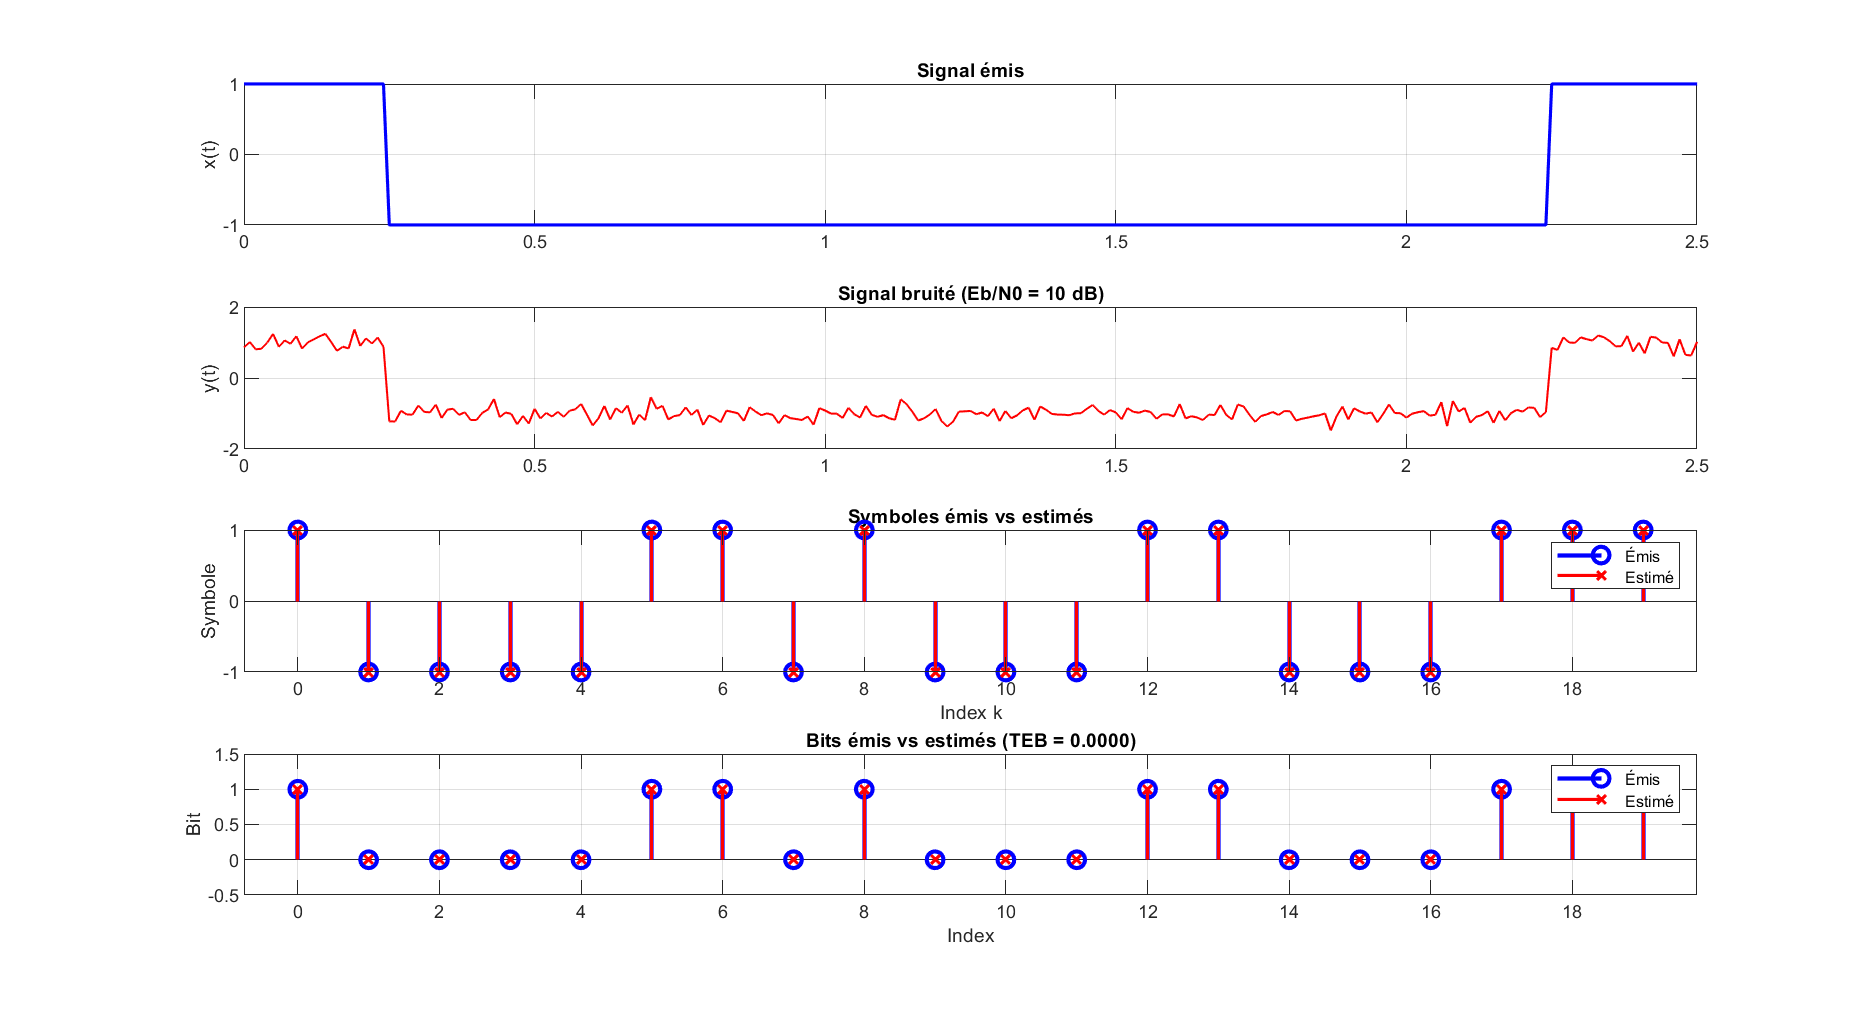
\includegraphics[width=0.95\textwidth]{../images/Q11_Q15_chaine_complete.png}
    \caption{Chaîne complète : émetteur, canal, récepteur}
    \label{fig:chaine_complete}
\end{figure}

\newpage

\section{Partie 3 : Performances}

\subsection{Taux d'Erreur Binaire (Q16)}

Le TEB mesure la qualité de la transmission.

\subsubsection{Définition}

\begin{equation}
    TEB = \frac{\text{nombre de bits mal transmis}}{\text{nombre total de bits émis}}
\end{equation}

\subsubsection{TEB théorique pour BPSK}

\begin{equation}
    TEB_{theo} = \frac{1}{2} \text{erfc}\left(\sqrt{\frac{E_b}{N_0}}\right)
\end{equation}

\subsection{Influence du filtre (Q17)}

Différents filtres de mise en forme ont des performances différentes en présence de bruit.

\textbf{Observations :}
\begin{itemize}
    \item Le filtre NRZ offre de bonnes performances
    \item Le filtre RZ a une énergie réduite (facteur 1/2)
    \item Le filtre biphase a une énergie constante mais une bande plus large
\end{itemize}

\subsection{Influence du dictionnaire (Q18)}

La taille du dictionnaire $M$ influence directement les performances.

\textbf{Résultats :}
\begin{itemize}
    \item $M = 2$ : meilleures performances (TEB le plus faible)
    \item $M = 4$ : performances intermédiaires
    \item $M = 8$ : performances dégradées (plus d'énergie nécessaire)
\end{itemize}

\begin{figure}[H]
    \centering
    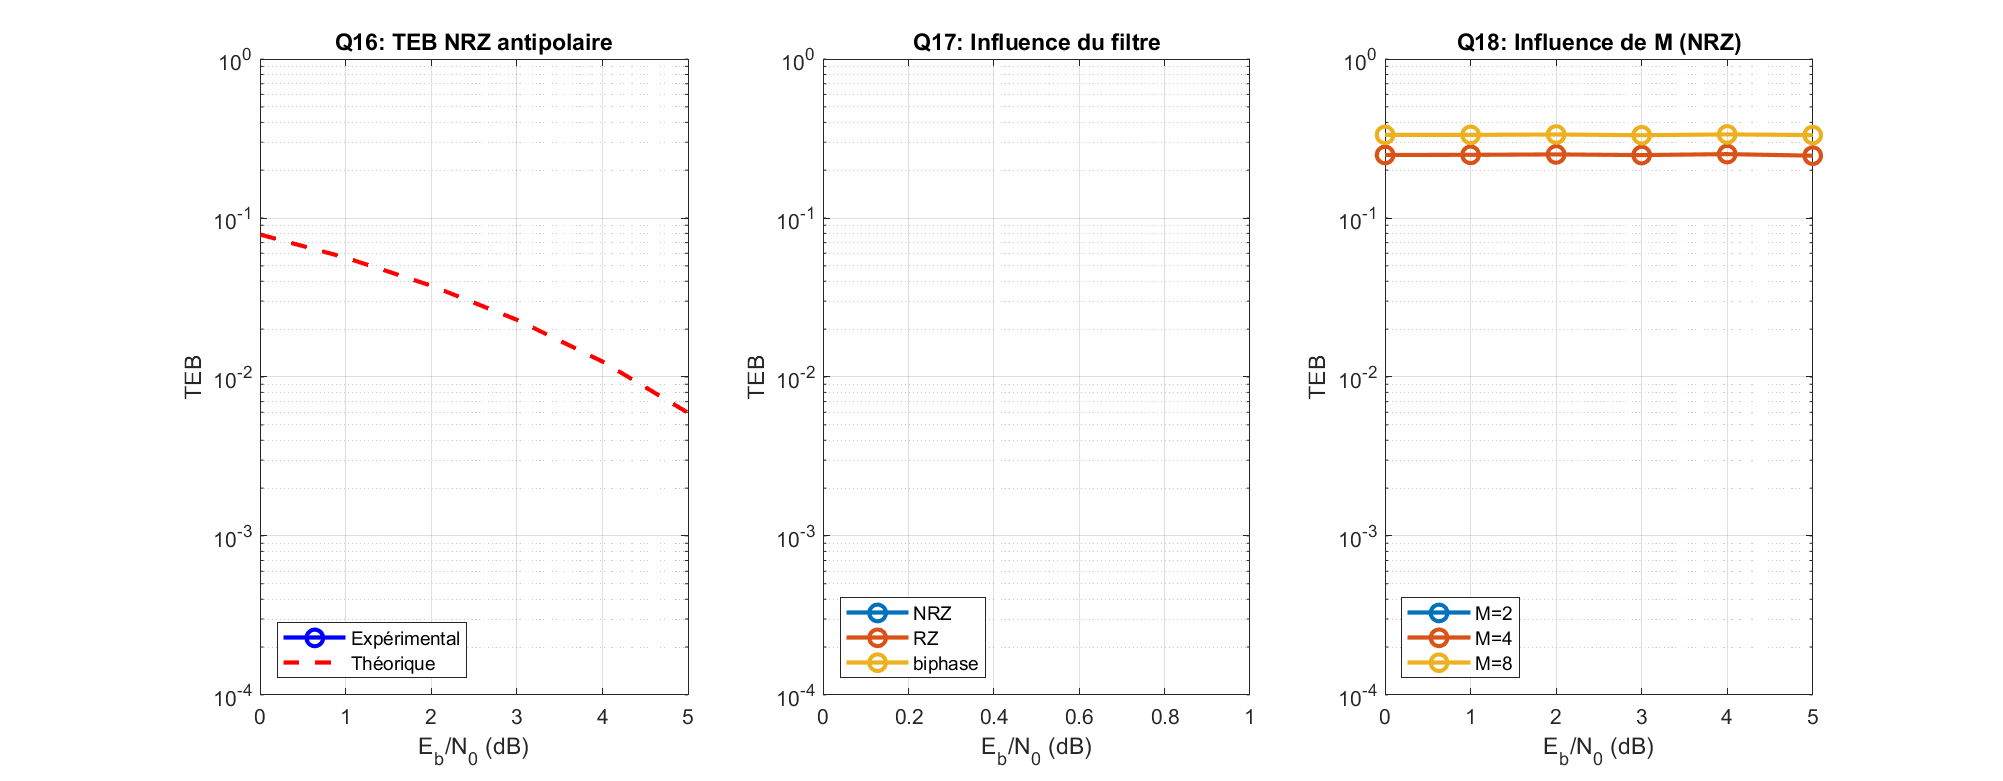
\includegraphics[width=0.95\textwidth]{../images/Q16_Q17_Q18_TEB.png}
    \caption{Performances : TEB en fonction de $E_b/N_0$}
    \label{fig:performances}
\end{figure}

\newpage

\section{Partie 4 : Transmission en bande modulée}

\subsection{Émetteur modulé (Q19)}

La modulation permet de transposer le signal en bande de base vers une fréquence porteuse.

\subsubsection{Principe}

Le signal modulé s'écrit :

\begin{equation}
    e(t) = I(t) \cos(2\pi f_0 t) - Q(t) \sin(2\pi f_0 t)
\end{equation}

où :
\begin{itemize}
    \item $I(t)$ : composante en phase (partie réelle des symboles)
    \item $Q(t)$ : composante en quadrature (partie imaginaire des symboles)
    \item $f_0$ : fréquence porteuse
\end{itemize}

\subsubsection{Symboles complexes}

Les symboles sont représentés dans le plan complexe :

\begin{equation}
    \alpha_k = a_k^I + j \cdot a_k^Q
\end{equation}

\subsection{Canal modulé (Q20)}

Le canal ajoute un bruit au signal modulé, identique au cas bande de base.

\subsection{Récepteur modulé (Q21)}

Le récepteur démodule le signal en multipliant par les porteuses en phase et en quadrature.

\subsubsection{Démodulation}

\begin{align}
    r_I(t) &= r(t) \cdot 2\cos(2\pi f_0 t) \\
    r_Q(t) &= -r(t) \cdot 2\sin(2\pi f_0 t)
\end{align}

Après filtrage passe-bas, on récupère $I(t)$ et $Q(t)$.

\begin{figure}[H]
    \centering
    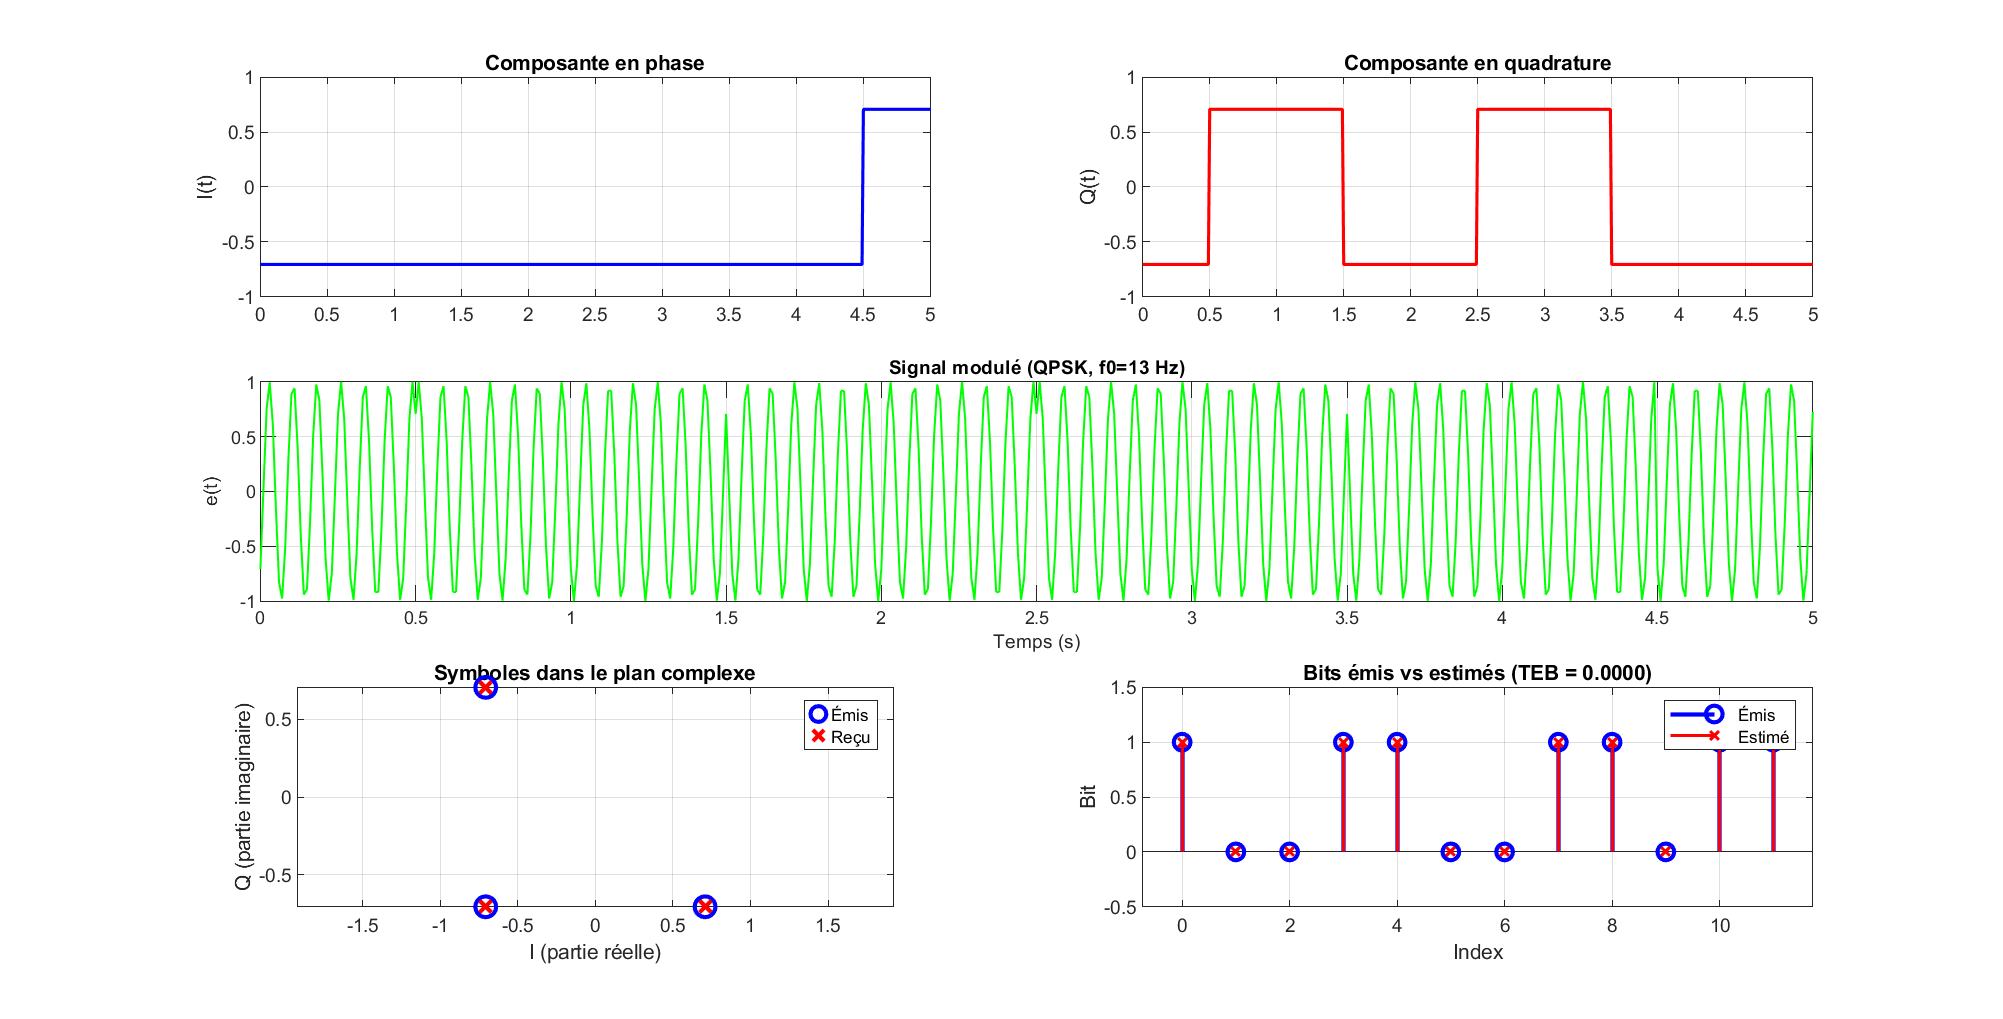
\includegraphics[width=0.95\textwidth]{../images/Q19_Q21_modulation.png}
    \caption{Modulation : composantes I/Q, signal modulé, plan complexe}
    \label{fig:modulation}
\end{figure}

\newpage

\subsection{Comparaison des modulations (Q22-Q24)}

\subsubsection{Q22 : Plan complexe}

Les différentes modulations se distinguent par la position de leurs symboles dans le plan complexe.

\textbf{Modulations étudiées :}
\begin{itemize}
    \item \textbf{BPSK} : 2 symboles sur l'axe réel
    \item \textbf{QPSK} : 4 symboles aux coins d'un carré
    \item \textbf{8-PSK} : 8 symboles sur un cercle
\end{itemize}

\begin{figure}[H]
    \centering
    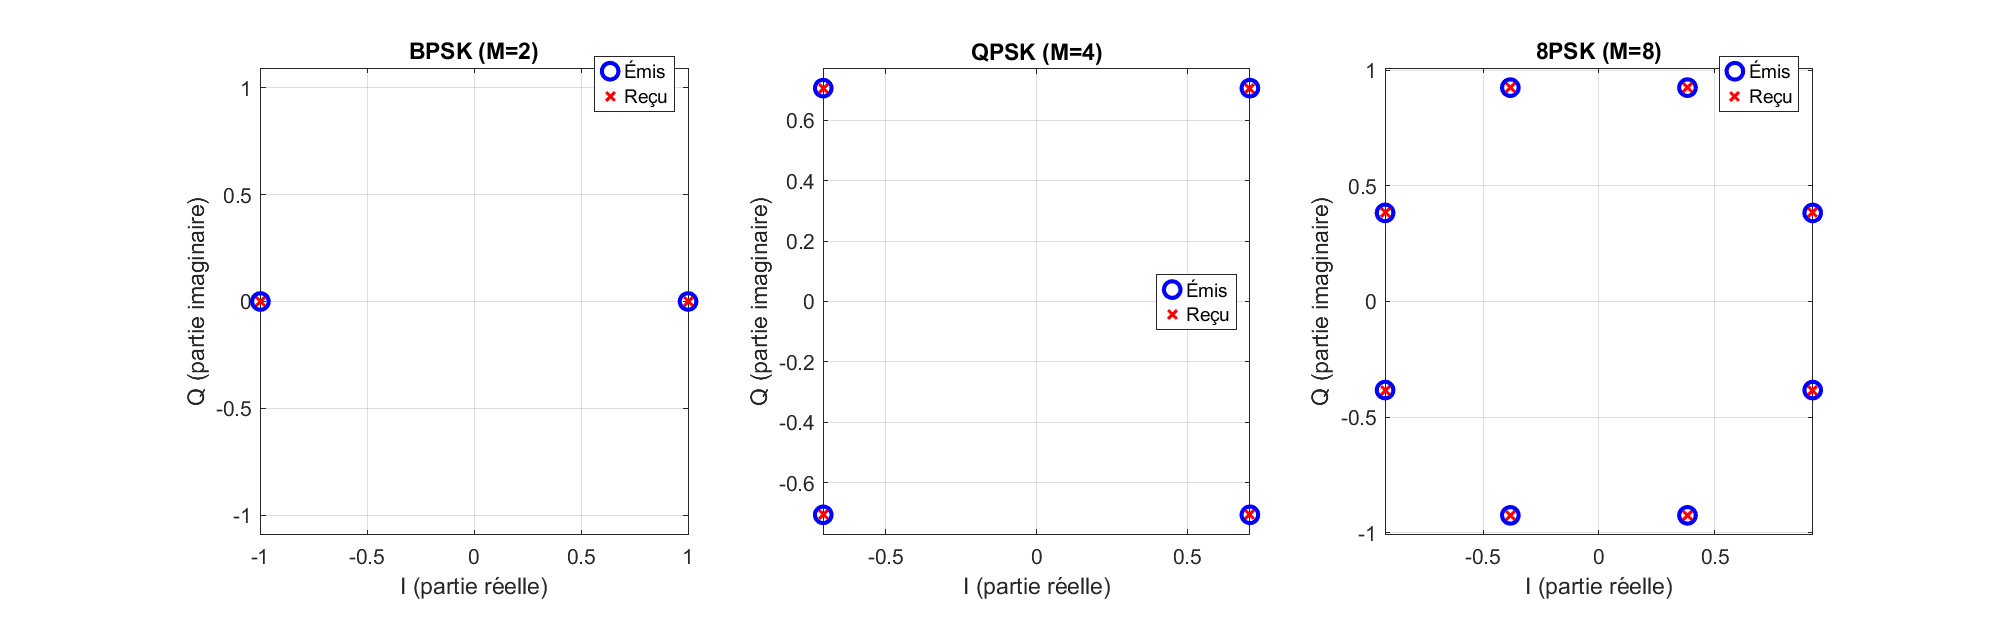
\includegraphics[width=0.95\textwidth]{../images/Q22_plan_complexe.png}
    \caption{Q22 : Symboles dans le plan complexe pour différentes modulations}
    \label{fig:plan_complexe}
\end{figure}

\subsubsection{Q23 : Densité Spectrale de Puissance}

La DSP permet d'analyser l'occupation spectrale de chaque modulation.

\begin{figure}[H]
    \centering
    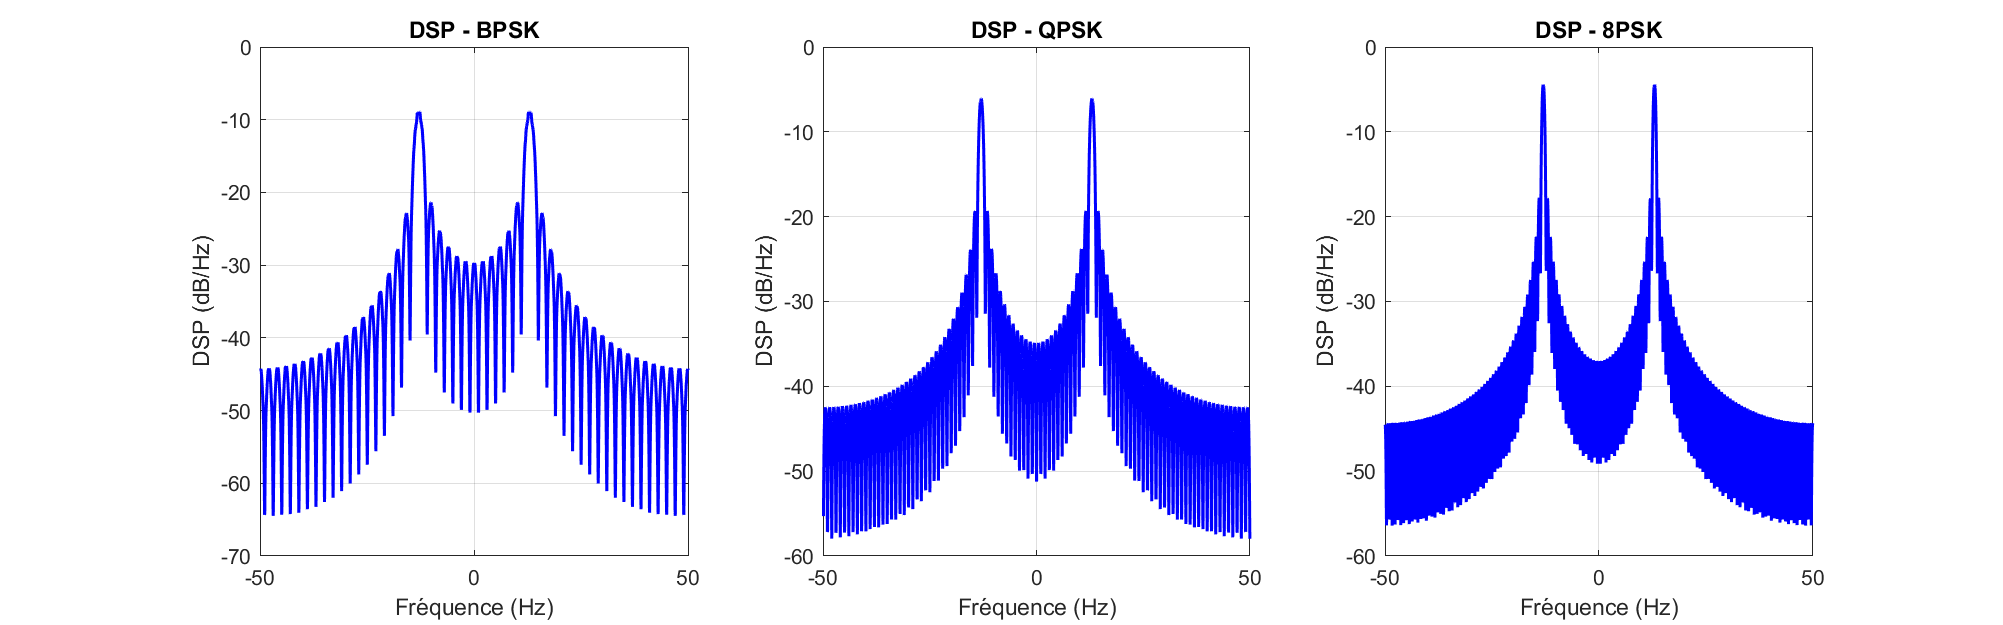
\includegraphics[width=0.95\textwidth]{../images/Q23_DSP.png}
    \caption{Q23 : DSP des signaux modulés}
    \label{fig:dsp}
\end{figure}

\subsubsection{Q24 : Performances comparées}

Le TEB permet de comparer les performances des différentes modulations.

\textbf{Résultats :}
\begin{itemize}
    \item BPSK et QPSK ont les mêmes performances (même distance entre symboles)
    \item 8-PSK a des performances dégradées (symboles plus proches)
    \item Les courbes expérimentales suivent bien la théorie
\end{itemize}

\begin{figure}[H]
    \centering
    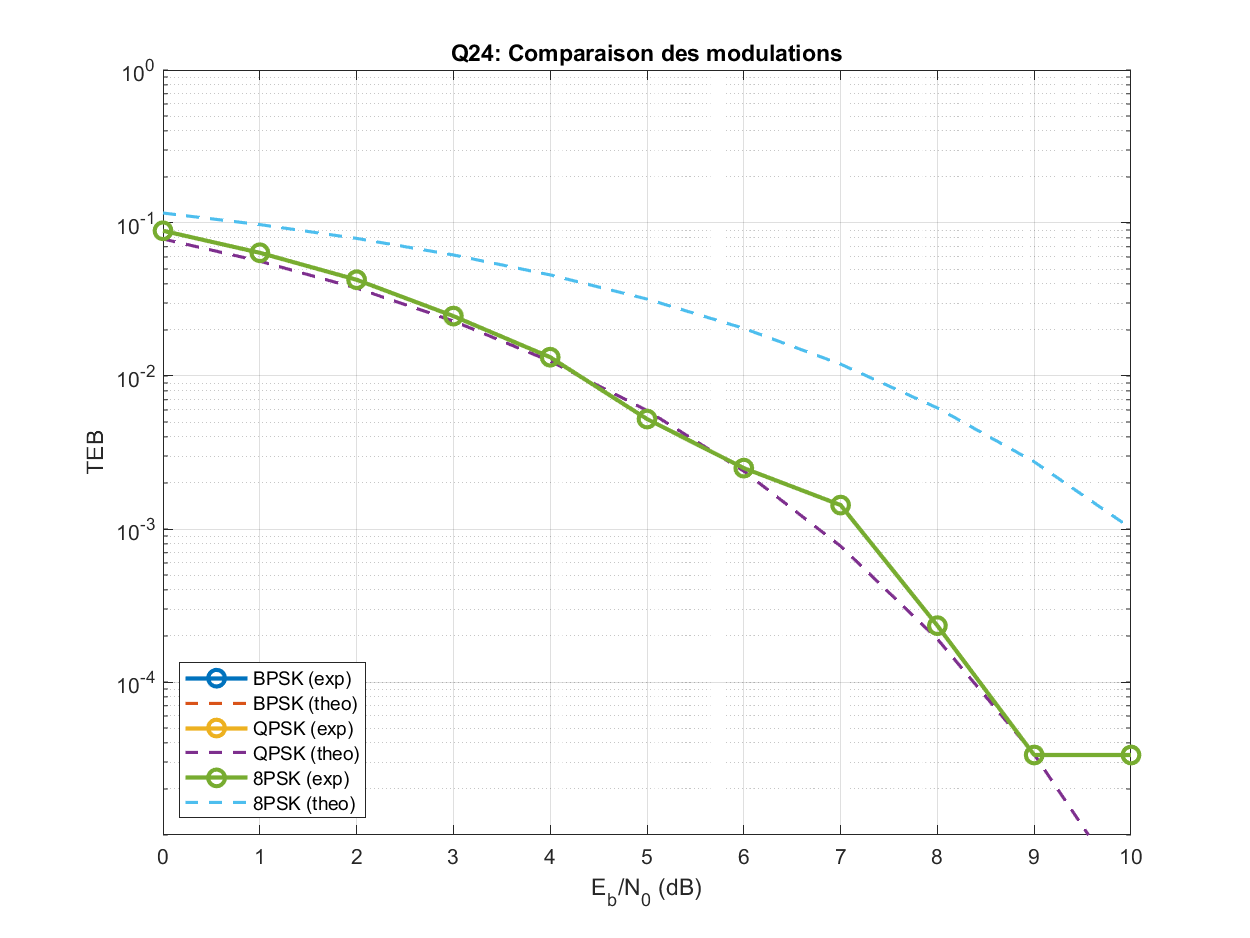
\includegraphics[width=0.8\textwidth]{../images/Q24_TEB_modulations.png}
    \caption{Q24 : TEB des différentes modulations}
    \label{fig:teb_modulations}
\end{figure}

\newpage

\subsection{Analyse spectrale (Q8)}

L'analyse spectrale permet de déterminer si un signal est en bande de base et d'estimer sa largeur de bande.

\subsubsection{Définition}

Un signal est dit \textbf{en bande de base} si son spectre est centré autour de la fréquence nulle (0 Hz) et ne contient pas de composante haute fréquence.

\subsubsection{Densité spectrale de puissance (DSP)}

La DSP est calculée par :

\begin{equation}
    S_x(f) = \mathcal{F}\{R_x(\tau)\}
\end{equation}

où $R_x(\tau)$ est la fonction d'autocorrélation.

\subsubsection{Largeur de bande}

La largeur de bande peut être estimée visuellement ou calculée comme la bande contenant 99\% de la puissance du signal.

\subsection{Influence du dictionnaire (Q9)}

Cette question étudie l'influence du type de dictionnaire et du filtre de mise en forme sur la largeur de bande.

\subsubsection{Observations attendues}

\begin{itemize}
    \item Le filtre de mise en forme a un impact majeur sur la largeur de bande
    \item Le dictionnaire (M-aire, antipolaire, unipolaire) influence principalement l'énergie, pas la bande
    \item Le filtre NRZ a une bande plus large que le filtre RCS
\end{itemize}

\subsection{Influence du dictionnaire M-aire (Q10)}

On étudie l'influence de la taille $M$ du dictionnaire sur la largeur de bande.

\subsubsection{Résultats attendus}

Pour un même filtre (par exemple NRZ) :
\begin{itemize}
    \item La période symbole $T$ augmente avec $M$ (car $T = m/D_b$ et $m = \log_2(M)$)
    \item La largeur de bande diminue quand $M$ augmente (car $BW \propto 1/T$)
    \item Compromis : plus de symboles $\Rightarrow$ moins de bande mais plus d'énergie par bit
\end{itemize}

\newpage

\section*{Conclusion}
\addcontentsline{toc}{section}{Conclusion}

Ce projet nous a permis d'étudier de manière exhaustive une chaîne de communication numérique complète, depuis l'émission jusqu'à la réception, en passant par un canal bruité.

\subsection*{Principaux résultats}

\textbf{Partie 1 : L'émetteur}
\begin{itemize}
    \item Implémentation réussie de la conversion bits/symboles avec différents dictionnaires
    \item Maîtrise de quatre types de filtres de mise en forme (NRZ, RZ, biphase, RCS)
    \item Calcul de l'énergie moyenne par bit pour différentes configurations
\end{itemize}

\textbf{Partie 2 : Canal et récepteur}
\begin{itemize}
    \item Modélisation d'un canal AWGN avec contrôle du rapport $E_b/N_0$
    \item Implémentation d'un récepteur optimal avec filtre adapté
    \item Décision par distance minimale pour estimer les symboles
\end{itemize}

\textbf{Partie 3 : Performances}
\begin{itemize}
    \item Calcul du TEB expérimental et comparaison avec la théorie
    \item Analyse de l'influence du filtre sur les performances
    \item Étude de l'impact de la taille du dictionnaire $M$ sur le TEB
    \item Validation : les courbes expérimentales suivent bien la théorie
\end{itemize}

\textbf{Partie 4 : Transmission en bande modulée}
\begin{itemize}
    \item Implémentation de modulations numériques (BPSK, QPSK, 8-PSK)
    \item Analyse des symboles dans le plan complexe
    \item Étude de la densité spectrale de puissance
    \item Comparaison des performances des différentes modulations
\end{itemize}

\subsection*{Observations clés}

\begin{enumerate}
    \item \textbf{Compromis énergie/bande :} Plus $M$ augmente, plus l'énergie par bit augmente, mais la bande passante diminue.
    
    \item \textbf{Filtre adapté :} Le récepteur optimal utilise un filtre adapté $h_r(t) = h_e(T-t)$ qui maximise le rapport signal/bruit.
    
    \item \textbf{Performances :} Le TEB diminue exponentiellement avec $E_b/N_0$, conformément à la théorie.
    
    \item \textbf{Modulations :} BPSK et QPSK offrent les mêmes performances, tandis que 8-PSK est moins robuste au bruit.
\end{enumerate}

\subsection*{Compétences acquises}

Ce projet nous a permis de :
\begin{itemize}
    \item Maîtriser les concepts fondamentaux des communications numériques
    \item Implémenter une chaîne de transmission complète sous MATLAB
    \item Analyser les performances d'un système de communication
    \item Comprendre les compromis entre efficacité spectrale et robustesse
    \item Valider expérimentalement les résultats théoriques
\end{itemize}

\subsection*{Perspectives}

Ce travail constitue une base solide pour l'étude de systèmes plus avancés :
\begin{itemize}
    \item Codes correcteurs d'erreurs (codes de Hamming, codes convolutifs, turbo-codes)
    \item Égalisation pour canaux à trajets multiples
    \item Modulations adaptatives (AMC - Adaptive Modulation and Coding)
    \item Systèmes MIMO (Multiple-Input Multiple-Output)
    \item OFDM (Orthogonal Frequency Division Multiplexing)
\end{itemize}

\vspace{1cm}

\textbf{Conclusion finale :} Ce projet nous a permis de comprendre en profondeur le fonctionnement d'une chaîne de communication numérique et de valider expérimentalement les concepts théoriques étudiés en cours. Les résultats obtenus sont conformes à la théorie et démontrent l'importance du choix des paramètres (filtre, modulation, dictionnaire) sur les performances du système.

\end{document}
